% \documentclass[preprint,12pt]{elsarticle}
\documentclass[preprint,review,12p,times]{elsarticle}
% \documentclass[times, review, 10pt]{elsarticle}

%% Use the option review to obtain double line spacing
%% \documentclass[authoryear,preprint,review,12pt]{elsarticle}

%% Use the options 1p,twocolumn; 3p; 3p,twocolumn; 5p; or 5p,twocolumn
%% for a journal layout:
%% \documentclass[final,1p,times]{elsarticle}
% \documentclass[final,1p,times,twocolumn]{elsarticle}
%% \documentclass[final,3p,times]{elsarticle}
%% \documentclass[final,3p,times,twocolumn]{elsarticle}
%% \documentclass[final,5p,times]{elsarticle}
%% \documentclass[final,5p,times,twocolumn]{elsarticle}

%% For including figures, graphicx.sty has been loaded in
%% elsarticle.cls. If you prefer to use the old commands
%% please give \usepackage{epsfig}

\usepackage{amssymb}
\usepackage{amsmath}
\usepackage{cases}
\usepackage{booktabs}
\usepackage{makecell}
\usepackage{tabularx}
\usepackage{multirow}
\usepackage{array}

\usepackage{textcomp}
\usepackage{stfloats}
\usepackage{url}
\usepackage{graphicx}
\usepackage{booktabs}
\usepackage{xcolor}
\usepackage{colortbl}
\usepackage{changepage}
\usepackage{algorithm}
\usepackage{algpseudocode}
\usepackage{soul}
\usepackage{float}
\usepackage{placeins}
% Keep floats close to their discussion and allow text to share the page.
\renewcommand{\topfraction}{0.90}
\renewcommand{\bottomfraction}{0.85}
\renewcommand{\textfraction}{0.10}
\renewcommand{\floatpagefraction}{0.85}
\setcounter{topnumber}{3}
\setcounter{bottomnumber}{2}
\setcounter{totalnumber}{5}
\setlength{\textfloatsep}{12pt plus 2pt minus 2pt}
\setlength{\floatsep}{10pt plus 2pt minus 2pt}
\setlength{\intextsep}{12pt plus 2pt minus 2pt}
\makeatletter
\setlength{\@fptop}{0pt}
\setlength{\@fpsep}{12pt}
\setlength{\@fpbot}{0pt plus 1fil}
\makeatother
\raggedbottom
% \usepackage[hidelinks]{hyperref}

%% The lineno packages adds line numbers. Start line numbering with
%% \begin{linenumbers}, end it with \end{linenumbers}. Or switch it on
%% for the whole article with \linenumbers.
%% \usepackage{lineno}

\journal{Image and Vision Computing}

\linespread{1.1}
\begin{document}

\begin{center}
    {\Large\bfseries Supplementary Material for Chain-Structured Binary Neural Architecture Search for Efficient Visual Recognition across Platforms\par}
\end{center}
\vspace{1em}

This supplementary material provides the experimental settings and analyses supporting the two-stage FlashNAS-BNN framework. We first specify the training, search, and latency measurement protocols, then describe the hardware-aware algorithm and the supplementary accuracy--OPs selection rule. The remaining sections examine the transfer from short-training accuracy to final architecture selection, explain the reported model configurations, and evaluate CLE across candidate-set sizes and repeated searches.

\section{Experimental Setup and Measurement Protocol}
\label{sec:detailed_latency_benchmark}

\subsection{\textcolor{red}{Training hyperparameters}}
\label{sec:training_hyperparameters}

\textcolor{red}{Table~\ref{tab:training_hyperparameters} summarizes the final training of selected architectures, following the procedures described in Section 4.2.3 of the main manuscript. ImageNet models use the two-phase ReActNet recipe~\cite{Liu2020}, with 128 epochs per phase by default, giving 256 total epochs. ImageNet-1000 additionally uses 256 epochs per phase, giving 512 total epochs: the shorter schedule supports comparisons with cell-based NAS methods, while the longer schedule supports comparisons with manually designed models and NAS-BNN. CIFAR models use 600 epochs of direct weight and activation quantization with the BATS hyperparameters~\cite{Bulat2020}. These schedules determine the reported final accuracies; the 25-epoch runs used to label architectures for CIF-Net serve a separate role during predictor construction.}

\begin{table}[!htbp]
    \centering
    \caption{\textcolor{red}{Training hyperparameters for the searched architectures on ImageNet and CIFAR.}}
    \label{tab:training_hyperparameters}
    \small
    {\color{red}
    \begin{tabularx}{\textwidth}{>{\raggedright\arraybackslash}p{0.24\textwidth} >{\raggedright\arraybackslash}X >{\raggedright\arraybackslash}X}
    \toprule
    Item & ImageNet-100/1000 & CIFAR-10/100 \\
    \midrule
    Task & Image classification & Image classification \\
    Optimizer & Adam & Adam \\
    Batch size & 256 & 256 \\
    Initial learning rate & $1.25\times10^{-3}$ per phase & $10^{-3}$ \\
    Learning-rate scheduler & Cosine decay per phase & Cosine decay \\
    Training procedure & Two-phase ReActNet recipe & Direct weight and activation quantization \\
    Training epochs & 128 per phase; also 256 per phase for ImageNet-1000 & 600 \\
    Total training epochs & 256; also 512 for ImageNet-1000 & 600 \\
    Weight decay & $10^{-5}$ in phase 1; $0$ in phase 2 & 0 \\
    Training seed & 1234 & 1234 \\
    \bottomrule
    \end{tabularx}}
\end{table}

\FloatBarrier
\subsection{\textcolor{red}{Search hyperparameters}}
\label{sec:search_hyperparameters}

\textcolor{red}{The evolutionary settings in Table~\ref{tab:search_hyperparameters} follow NAS-BNN~\cite{Lin2025} in population size, crossover and mutation counts, and search budget. Each iteration generates offspring and updates the candidate population using predicted accuracy and operation cost. The 20-iteration budget therefore counts evolutionary updates, rather than training epochs for each candidate; CIF-Net label generation and final model training have their own budgets. The table reports the default search seed, while Section~\ref{sec:architecture_selection_repeatability} specifies the three seeds used to examine repeated-search performance.}

\begin{table}[!htbp]
    \centering
    \caption{\textcolor{red}{Architecture search hyperparameters.}}
    \label{tab:search_hyperparameters}
    \small
    {\color{red}
    \begin{tabularx}{\textwidth}{>{\raggedright\arraybackslash}p{0.55\textwidth} X}
    \toprule
    Item & Setting \\
    \midrule
    Initial population size ($N_{\text{init}}$) & 512 \\
    Crossover offspring ($N_{\text{cross}}$) & 128 \\
    Mutation offspring ($N_{\text{mut}}$) & 128 \\
    Mutation probability ($p_{\text{mut}}$) & 0.2 \\
    Candidate selection size ($N_{\text{cand}}$) & 500 \\
    Evolutionary search budget & 20 iterations \\
    Search seed & 2024 \\
    \midrule
    ImageNet-100/1000 OP constraint & $(83$--$88)\times10^6$ OPs \\
    CIFAR-10/100 OP constraint & $(0.11$--$0.18)\times10^8$ OPs \\
    \bottomrule
    \end{tabularx}}
\end{table}

\textcolor{red}{The OP intervals in Table~\ref{tab:search_hyperparameters} define the feasible computational budgets for the ImageNet-100/1000 and CIFAR-10/100 experiments. We calculate operation cost as $\mathrm{OP}=\mathrm{BOPs}/64+\mathrm{QOPs}/8+\mathrm{FLOPs}$, using the target dataset's input resolution and classification head. Consequently, sharing a backbone across two datasets does not require identical total OP counts. In the controlled selection analysis in Section~\ref{sec:supp_accuracy_ops_transfer}, both accuracy criteria use the same target-dataset OP counts and feasibility interval, so their comparison reflects the accuracy signal rather than a change in computational budget.}
% Record check: the reported CIFAR interval and A*/B*/C* costs must be
% checked against matching profiling records; no new profiling was performed
% during this wording revision. The former literature/TBD paragraph is
% preserved in the revision archive rather than presented as an experiment.

\FloatBarrier
\subsection{\textcolor{red}{Latency measurement protocol}}

\textcolor{red}{All measured inference latencies in the main manuscript and this supplement follow the protocol below, including platform comparisons and evaluations of architectures selected during search. For the ImageNet-100 comparison, BNAS, EBNAS, and NAS-BNN were trained on ImageNet-100 using their respective codebases and method-specific procedures. Their accuracies therefore refer to this dataset, while the training procedures remain specific to each method. On FPGA, the baselines and FlashNAS-BNN use the same accelerator implementation, keeping the deployment basis consistent across the reported models.}
\begin{itemize}
    \item \textbf{Workload:} Measurements use batches of 32 images at an input resolution of $224\times224$. Latency is normalized per image by dividing the measured batch inference time by the batch size, so the reported values describe the specified batched workload.
    \item \textbf{Software:} The training environment includes PyTorch 2.6.0 and CUDA Toolkit 12.6. CPU/GPU profiling uses Huawei's Noah's Bolt v1.5.2~\cite{Huawei2020}, with the default OpenCL backend for GPU inference. \textcolor{red}{The FPGA accelerator follows Zhang et al.~\cite{Zhang2025} and uses Vitis HLS 2022.1 and Vivado 2022.1.}
    \item \textbf{Timing boundary:} Timing begins when a prepared input tensor is supplied to the platform runtime and ends when the corresponding model output is available. Host-side image preprocessing is excluded. Synchronization before execution and after inference completion ensures that asynchronous device work is included in the timed interval.
    \item \textbf{Repetitions:} Each model undergoes 20 warm-up iterations followed by 50 timed iterations. \textcolor{red}{We report the mean $\pm$ standard deviation (SD) of the 50 per-image latency values in ms/image. This SD describes timing variability for one selected architecture; variability across independent searches is summarized separately in Section~\ref{sec:architecture_selection_repeatability}.}
    \item \textbf{Hardware:} \textcolor{red}{CPU inference uses one Cortex-X4 thread at 3.3~GHz with Bolt's \texttt{CPU\_AFFINITY\_HIGH\_PERFORMANCE} policy. The Mali-G77 MP9 GPU runs at 836~MHz, and the XC7VX690T FPGA runs at 180~MHz. CPU and GPU use their highest frequency operating points, with an external fan limiting thermal effects during benchmarking.}
\end{itemize}

\section{Two-stage search algorithm}
\label{sec:supp_search_algorithm}

Algorithm~\ref{alg:flashnas} separates platform-independent exploration from platform-specific selection. Stage I evolves architectures using CIF-Net accuracy predictions and OPs, retaining a candidate set that can be reused across target platforms within the same search setting. Stage II then evaluates latency only within this set: small pools are measured directly, whereas larger pools use CLE fitted from a measured subset. The final choice minimizes a normalized accuracy--latency objective for the target platform. This separation makes the candidate-generation process reusable while allowing different hardware latency inputs to produce different final selections.

\begingroup
\color{red}
\paragraph{Candidate representation and variation.}
An architecture is an ordered collection of stage-wise depth, channel-width, and convolution choices from the main manuscript's search space. Crossover combines architectural choices from two parents, whereas mutation perturbs choices in one parent. Changes in depth require the layer sequence and stage transitions to remain consistent with the backbone topology. The offspring counts are separate: $N_{\text{cross}}=128$ and $N_{\text{mut}}=128$ per evolutionary update. These counts specify how many offspring are generated, rather than probabilities of applying the two operators. Candidate generation must preserve valid stage boundaries and allowed architectural choices, and candidates must satisfy the benchmark-specific OP budget in Table~\ref{tab:search_hyperparameters}.

\paragraph{Evaluation and non-dominated filtering.}
For each candidate, operation cost is calculated analytically and accuracy is predicted by the fixed CIF-Net used for the search. Thus, a search iteration does not train the candidate networks. For the objective pair $(-\widehat{Acc},OP)$, architecture $a$ dominates $b$ when $\widehat{Acc}(a)\geq\widehat{Acc}(b)$ and $OP(a)\leq OP(b)$, with at least one strict inequality. Non-dominated filtering compares these two quantities without a scalar weight. The parent--offspring update in Algorithm~\ref{alg:flashnas} repeats for 20 iterations, after which the retained set is supplied to platform-specific selection. Equation (\ref{eq:supp_ops_selection}) instead describes the subsequent accuracy--OPs selection of reference variants; its coefficient does not govern evolutionary filtering.

\paragraph{Platform-specific selection and final training.}
For a fixed dataset, search space, and search run, the same Stage-I pool is reused across target platforms. With at most $N_{\mathrm{thr}}=250$ candidates, Stage II measures the entire pool; for larger pools, it fits CLE using a measured subset and estimates latency for all candidates. Min--max normalization uses the full retained pool, with latency extrema calculated separately for each platform. Stage II minimizes the weighted accuracy--latency objective over this fixed pool, without further crossover or mutation. Only the selected architectures then undergo the final training schedules in Section 1.1. Supplementary Section 7.1 explains the threshold, and Section 6 reports the selection weights and model mapping.
\endgroup

\begin{algorithm}
\caption{\linespread{1.0}\selectfont
Chain-Structured Binary Neural Architecture Search for Efficient Visual Recognition across Platforms}
\label{alg:flashnas}
\small
\setlength{\baselineskip}{10pt}
\begin{algorithmic}[1]
\renewcommand{\algorithmicrequire}{\textbf{Input:}}
\renewcommand{\algorithmicensure}{\textbf{Output:}}

\Require Search space $\mathcal{A}$; target platform $p\in\mathcal{P}$; population size $N_{\text{init}}$; iterations $iter$;
crossover offspring $N_{\text{cross}}$; mutation offspring $N_{\text{mut}}$; mutation probability $p_{\text{mut}}$; selection size $N_{\text{cand}}$;
Stage-II threshold $N_{\text{thr}}$;
non-dominated filtering $\mathrm{ND(\cdot)}$;
Stage-II accuracy weight $w_{\mathrm{Lat}}\in[0,1]$;
accuracy predictor $\widehat{Acc}(\cdot)$ (CIF-Net); latency estimator $\hat{T}(\cdot,p)$ (CLE); measurement routine $T(\cdot,p)$.
\Ensure $a^*=\arg\min_{a\in\mathcal{A}_{\text{opt}}}\tilde{F}(a;p)$.

\State $\mathcal{G}_0 \gets \textbf{Sample}(\mathcal{A},N_{\text{init}})$
\For{$t=1$ \textbf{to} $iter$}
  \State $\mathcal{O}^{\mathrm{cross}}_t\gets\mathrm{Crossover}(\mathcal{G}_{t-1},N_{\text{cross}})$
  \State $\mathcal{O}^{\mathrm{mut}}_t\gets\mathrm{Mutate}(\mathcal{G}_{t-1},N_{\text{mut}},p_{\text{mut}})$
  \State $\mathcal{U}_t\gets\mathcal{G}_{t-1}\cup\mathcal{O}^{\mathrm{cross}}_t\cup\mathcal{O}^{\mathrm{mut}}_t$
  \ForAll{$a\in\mathcal{U}_t$} \State Compute $OP(a)$; predict $\widehat{Acc}(a)$ \EndFor
  \State $\mathcal{G}_t \gets \mathrm{Select}\!\left(\mathrm{ND}\!\left(\{(a,-\widehat{Acc}(a),OP(a))~|~a\in\mathcal{U}_t\}\right),N_{\text{cand}}\right)$
\EndFor
\State $\mathcal{A}_{\text{opt}}\gets\mathcal{G}_{iter}$ 

\If{$|\mathcal{A}_{\text{opt}}|\le N_{\text{thr}}$}
  \ForAll{$a\in\mathcal{A}_{\text{opt}}$} \State Measure $T(a,p)$; set $\hat{T}(a,p)\leftarrow T(a,p)$ \EndFor
\Else
  \State $\mathcal{S}\gets\textbf{Sample}(\mathcal{A}_{\text{opt}},N_{\text{train}})$; measure $\{T(a,p)\}_{a\in\mathcal{S}}$
  \State Train CLE on $\{(a,p,T(a,p))~|~a\in\mathcal{S}\}$; predict $\hat{T}(a,p)$ for all $a\in\mathcal{A}_{\text{opt}}$
\EndIf

\State Compute $\widehat{Acc}_{\min},\widehat{Acc}_{\max}$ over $\{\widehat{Acc}(a)\}_{a\in\mathcal{A}_{\text{opt}}}$ and $\hat{T}_{\min}(p),\hat{T}_{\max}(p)$ over $\{\hat{T}(a,p)\}_{a\in\mathcal{A}_{\text{opt}}}$
\ForAll{$a\in\mathcal{A}_{\text{opt}}$}
  \State $\tilde{f}_1(a)=\frac{\widehat{Acc}_{\max}-\widehat{Acc}(a)}{\widehat{Acc}_{\max}-\widehat{Acc}_{\min}+\epsilon}$;~~
         $\tilde{f}_2(a,p)=\frac{\hat{T}(a,p)-\hat{T}_{\min}(p)}{\hat{T}_{\max}(p)-\hat{T}_{\min}(p)+\epsilon}$
  \State $\tilde{F}(a;p)=w_{\mathrm{Lat}}\tilde{f}_1(a)+(1-w_{\mathrm{Lat}})\tilde{f}_2(a,p)$
\EndFor
\State \Return $a^*=\arg\min_{a\in\mathcal{A}_{\text{opt}}}\tilde{F}(a;p)$
\end{algorithmic}
\end{algorithm}

\subsection{\textcolor{red}{Supplementary accuracy--OPs selection criterion}}
\label{sec:supp_ops_selection}

\begingroup
\color{red}
Reference variants A--F complement the hardware-aware models by characterizing accuracy--OPs trade-offs without a device-latency objective. They are selected after Stage-I exploration from the OP-feasible Pareto candidate pool $\mathcal C$ of the corresponding search run. This supplementary rule uses the existing pool rather than rerunning architecture exploration for each coefficient. To combine accuracy and operation cost on comparable scales, we normalize both objectives over $\mathcal C$:
\begin{align}
\widetilde f_{\mathrm{acc}}(a)
&=\frac{\widehat{Acc}_{\max}-\widehat{Acc}(a)}
{\widehat{Acc}_{\max}-\widehat{Acc}_{\min}+\epsilon},\\
\widetilde f_{\mathrm{OP}}(a)
&=\frac{OP(a)-OP_{\min}}{OP_{\max}-OP_{\min}+\epsilon}.
\end{align}
The resulting weighted criterion selects the architecture that minimizes the combined accuracy loss and operation cost:
\begin{equation}
a^*_{\mathrm{OP}}(w_{\mathrm{OP}})
=\underset{a\in\mathcal C}{\arg\min}\,
\left[w_{\mathrm{OP}}\widetilde f_{\mathrm{acc}}(a)
+(1-w_{\mathrm{OP}})\widetilde f_{\mathrm{OP}}(a)\right],
\quad w_{\mathrm{OP}}\in[0,1].
\label{eq:supp_ops_selection}
\end{equation}
Increasing $w_{\mathrm{OP}}$ emphasizes predicted accuracy, while decreasing it emphasizes lower OPs within the feasible pool. At $w_{\mathrm{OP}}=1$, the operation-cost term vanishes and selection maximizes predicted accuracy subject to the pool's OP constraints, as used for F. This coefficient governs supplementary selection after Pareto filtering; it does not change Stage-I non-dominated screening or replace the Stage-II accuracy--latency weight $w_{\mathrm{Lat}}$. Table~\ref{tab:model_selection_config} records the model-specific settings, and Section~\ref{sec:supp_accuracy_ops_transfer} compares reduced-budget searches guided by measured short- and full-training accuracies.
\endgroup

\begingroup
\color{red}
\section{\textcolor{red}{CIF-Net training and cross-dataset evaluation}}

\label{sec:supp_predictor_groups}

\paragraph{Predictor construction and data provenance.}

We train CIF-Net separately for the ImageNet and CIFAR experiments, using 25-epoch accuracy labels from ImageNet-100 and CIFAR-100, respectively. Each predictor uses labels from 750 sampled architectures, divided into 80\% training and 20\% held-out sets, with offline preparation accounted for separately for each predictor. The corresponding predictor supplies the accuracy signal for Stage-I exploration. The predictor metrics in the main manuscript assess agreement with the short-training labels on which CIF-Net is fitted. Table~\ref{tab:epoch_transfer} evaluates how well short-training accuracy preserves architecture rankings across training budgets and datasets. Table~\ref{tab:acc_ops_oracle} tests the practical effect of this signal by comparing the final architectures obtained from short-training-guided and full-training-guided searches under the same reduced search budget and OP constraints.

\subsection{\textcolor{red}{Short-training versus full-training accuracy}}

\label{sec:supp_epoch_transfer}

To assess the labeling signal independently of CIF-Net fitting, we used three sampled sets of 100 architectures for each source dataset, ImageNet-100 and CIFAR-100, with architecture-sampling seeds 2024, 1234, and 42. These architectures were excluded from the predictor's training and validation partitions, and each seed-specific set remained fixed across the 15-, 20-, 25-, and 30-epoch source-dataset evaluations. The same architectures were fully trained on the target datasets to provide reference accuracies. ImageNet-100 supplied source accuracies for ImageNet-100 and ImageNet-1000, while CIFAR-100 supplied those for CIFAR-100 and CIFAR-10. Table~\ref{tab:epoch_transfer} separates within-dataset training-budget transfer from cross-dataset transfer, because the latter also changes the classification task.

The reference training used 256 total epochs for ImageNet-100 and 600 epochs for CIFAR. For both Tables~\ref{tab:epoch_transfer} and~\ref{tab:acc_ops_oracle}, ImageNet-1000 reference accuracies were obtained using the two-phase ReActNet recipe with 256 epochs per phase (512 epochs in total). The 256-total-epoch ImageNet-1000 schedule was not evaluated in these analyses. The sampling design for Table~\ref{tab:epoch_transfer} gives 300 architecture instances for each source dataset, with separate full-training tasks for its two corresponding target datasets. We computed each metric within a seed-specific set and then summarized the three values, rather than pooling all instances as distinct architectures. The resulting SD describes variation across sampled architecture sets. This sampling repetition is separate from the model-training seed in Table~\ref{tab:training_hyperparameters}, so it does not represent repeated training of every fixed architecture.
The budgets of 15, 20, 25, and 30 epochs denote the total short-training budget per architecture. All short-training runs on ImageNet and CIFAR use a single W1A1 phase (binary weights and activations) for the entire budget. For these evaluations, we retained the base training hyperparameters in Table~\ref{tab:training_hyperparameters} but shortened the training horizon and adjusted the learning-rate schedule to the corresponding budget. Each short-training result therefore comes from a budget-specific training run, rather than an intermediate checkpoint of the full-training schedule.

\paragraph{Rank and normalized-value agreement.}

For dataset pair $D_s\!\to\!D_t$, let $A_{i,s}^{(e)}$ denote architecture $i$'s source accuracy after $e$ epochs and $A_{i,t}^{(F)}$ its fully trained target accuracy. Kendall's $\tau_b$ and Spearman's $\rho$ compare how the same architectures are ordered by the two accuracy vectors. To also compare relative numerical values across training budgets and datasets, we define $z(x_i;\mathcal S)=[x_i-\min_{j\in\mathcal S}x_j]/[\max_{j\in\mathcal S}x_j-\min_{j\in\mathcal S}x_j+\epsilon]$ within each seed-specific architecture set $\mathcal S$. The corresponding measures are the min--max-normalized MSE and $R^2_{\mathrm{norm}}$:

\begin{equation}
\mathrm{MSE}_{\mathrm{mm}}^{(e,F)}=\frac{1}{|\mathcal S|}\sum_{i\in\mathcal S}\left[z(A_{i,s}^{(e)};\mathcal S)-z(A_{i,t}^{(F)};\mathcal S)\right]^2,
\end{equation}

\begin{equation}
R^2_{\mathrm{norm}}=1-\frac{\sum_{i\in\mathcal S}\left[z(A_{i,s}^{(e)};\mathcal S)-z(A_{i,t}^{(F)};\mathcal S)\right]^2}{\sum_{i\in\mathcal S}\left[z(A_{i,t}^{(F)};\mathcal S)-\overline{z(A_t^{(F)})}\right]^2}.
\end{equation}

Here $\mathrm{MSE}_{\mathrm{mm}}$ measures the mean squared difference between separately min--max-normalized accuracy vectors, while $R^2_{\mathrm{norm}}$ compares this discrepancy with variation in the normalized full-training reference. These quantities describe relative numerical agreement after removing location and scale differences, apart from the stabilizer $\epsilon$; they are not absolute target-accuracy prediction errors. They compare observed short- and full-training accuracies, whereas the main manuscript's MSE evaluates predictions against 25-epoch labels on the predictor's evaluation scale. The rank statistics are reported alongside them, together with $\mathrm{Recall@10}=|\mathrm{Top}_{10}(A_s^{(e)})\cap\mathrm{Top}_{10}(A_t^{(F)})|/10$ to measure overlap among high-performing architectures. Kendall's $\tau_b$ accounts for ties, and Top-10 membership uses a consistent tie-handling rule. This combination distinguishes global ordering, high-accuracy candidate retention, and normalized numerical agreement without treating normalization itself as evidence of rank transfer.

\begin{table}[!htbp]
\centering
\color{red}
\caption{Agreement between short-training source accuracy and full-training target accuracy across three sampling seeds, with 100 matched architectures per seed. Entries report the arithmetic mean, with SD in parentheses, for each metric.}
\label{tab:epoch_transfer}
\scriptsize
\setlength{\tabcolsep}{4pt}
\resizebox{\textwidth}{!}{%
\begin{tabular}{llccccc}
\toprule
Dataset pair & Epochs & Kendall $\tau_b$ $\uparrow$ & Spearman $\rho$ $\uparrow$ & $\mathrm{MSE}_{\mathrm{mm}}$ $\downarrow$ & $R^2_{\mathrm{norm}}$ $\uparrow$ & Recall@10 $\uparrow$ \\
\midrule
\multirow{4}{*}{\makecell[l]{ImageNet-100 \\ $\to$ ImageNet-100}}
& 15 & 0.65(0.04) & 0.81(0.03) & 0.032(0.005) & 0.66(0.04) & 0.60(0.05) \\
& 20 & 0.72(0.03) & 0.87(0.02) & 0.024(0.004) & 0.75(0.03) & 0.70(0.04) \\
& \textbf{25} & \textbf{0.79(0.03)} & \textbf{0.91(0.02)} & \textbf{0.017(0.003)} & \textbf{0.82(0.03)} & \textbf{0.80(0.03)} \\
& 30 & 0.82(0.02) & 0.93(0.01) & 0.014(0.002) & 0.85(0.02) & 0.83(0.03) \\
\midrule
\multirow{4}{*}{\makecell[l]{ImageNet-100 \\ $\to$ ImageNet-1000}}
& 15 & 0.53(0.05) & 0.72(0.04) & 0.070(0.008) & 0.30(0.05) & 0.47(0.06) \\
& 20 & 0.60(0.04) & 0.78(0.03) & 0.062(0.007) & 0.39(0.04) & 0.57(0.05) \\
& \textbf{25} & \textbf{0.65(0.04)} & \textbf{0.82(0.03)} & \textbf{0.054(0.006)} & \textbf{0.46(0.04)} & \textbf{0.67(0.04)} \\
& 30 & 0.68(0.03) & 0.84(0.02) & 0.049(0.005) & 0.51(0.03) & 0.70(0.04) \\
\midrule
\multirow{4}{*}{\makecell[l]{CIFAR-100 \\ $\to$ CIFAR-100}}
& 15 & 0.61(0.04) & 0.78(0.03) & 0.038(0.006) & 0.61(0.04) & 0.57(0.05) \\
& 20 & 0.70(0.03) & 0.85(0.03) & 0.027(0.004) & 0.72(0.03) & 0.67(0.04) \\
& \textbf{25} & \textbf{0.77(0.03)} & \textbf{0.90(0.02)} & \textbf{0.019(0.003)} & \textbf{0.80(0.03)} & \textbf{0.77(0.04)} \\
& 30 & 0.81(0.02) & 0.92(0.02) & 0.016(0.003) & 0.83(0.02) & 0.83(0.03) \\
\midrule
\multirow{4}{*}{\makecell[l]{CIFAR-100 \\ $\to$ CIFAR-10}}
& 15 & 0.58(0.04) & 0.75(0.04) & 0.065(0.007) & 0.38(0.05) & 0.50(0.05) \\
& 20 & 0.65(0.04) & 0.81(0.03) & 0.054(0.006) & 0.49(0.04) & 0.60(0.05) \\
& \textbf{25} & \textbf{0.69(0.03)} & \textbf{0.85(0.03)} & \textbf{0.044(0.005)} & \textbf{0.58(0.04)} & \textbf{0.70(0.04)} \\
& 30 & 0.71(0.03) & 0.87(0.02) & 0.040(0.004) & 0.62(0.03) & 0.73(0.03) \\
\bottomrule
\end{tabular}}
\end{table}

\noindent\textbf{Ranking comparison and choice of 25 epochs.}
At 25 epochs, Spearman correlation was 0.91 for ImageNet-100 and 0.90 for CIFAR-100, compared with 0.82 and 0.85 for their respective cross-dataset transfers (Table~\ref{tab:epoch_transfer}). Cross-dataset Recall@10 was 0.67 and 0.70, respectively, indicating partial retention of the full-training Top-10 architectures. The correlations describe association across the sampled architectures, while Top-10 overlap shows that membership among the highest-accuracy candidates changed. Together, these measurements indicate positive but incomplete agreement, with weaker transfer across datasets.

The budget comparison also shows why we retain 25 epochs for label generation. Moving from 20 to 25 epochs increased cross-dataset Spearman correlation by 0.04 for both ImageNet-100-to-ImageNet-1000 and CIFAR-100-to-CIFAR-10 transfer, whereas moving from 25 to 30 epochs added 0.02. The latter extension requires 20\% more training epochs per architecture. Thus, 25 epochs provides a labeling-budget versus agreement trade-off under the evaluated settings, rather than an optimality claim: 30 epochs still improved all five metrics in every dataset pair.

\subsection{\textcolor{red}{Accuracy--OPs search under a reduced budget}}
\label{sec:supp_accuracy_ops_transfer}

We compare Stage-I searches guided by measured 25-epoch source accuracy and full-training target accuracy under the same search space and target-dataset OP constraints from Section~\ref{sec:search_hyperparameters}. To keep full-training-guided search tractable, we reduce the initial population to $N_{\text{init}}=64$, generate $N_{\text{cross}}=18$ crossover and $N_{\text{mut}}=18$ mutation offspring, and perform $iter=1$ evolutionary update. We repeat both searches using seeds 2024, 1234, and 42. The accuracy signal is measured directly in each case, isolating short-training effects from CIF-Net prediction error; device latency is not part of this comparison.

Final selection uses the accuracy--OPs criterion in Eq.~(\ref{eq:supp_ops_selection}) with $w_{\mathrm{OP}}=1$, while Stage-I evolution retains accuracy--OPs Pareto filtering. Let $a^{25}_s$ and $a^F_s$ denote the architectures selected by the short-training-guided and full-training-guided searches for seed $s$, respectively. We evaluate both selected architectures using full-training target accuracy and target-dataset OPs. The paired accuracy difference is
\begin{equation}
\Delta\operatorname{Acc}_{F,s}
=\operatorname{Acc}_{F,D_t}(a^F_s)
-\operatorname{Acc}_{F,D_t}(a^{25}_s).
\end{equation}
Differences are calculated within each seed before their mean and sample standard deviation are computed across the three searches.

\begin{table}[!htbp]

\centering
\color{red}

\caption{Accuracy-guided search under a reduced evolutionary budget. Results are mean $\pm$ sample SD across three search seeds. Top-1 values are full-training target accuracies; $\Delta$Acc is the paired difference relative to full-training-guided search, in percentage points (pp).}

\label{tab:acc_ops_oracle}

\small

\resizebox{\textwidth}{!}{%
\begin{tabular}{llccc}

\toprule

Target dataset & Search accuracy signal & Full Top-1 (\%) $\uparrow$ & OPs ($10^8$) $\downarrow$ & $\Delta$Acc (pp) $\downarrow$ \\

\midrule

ImageNet-100 & 25-epoch accuracy & $81.65\pm0.15$ & $0.856\pm0.007$ & $0.11\pm0.06$ \\

& Full-training accuracy & $81.76\pm0.12$ & $0.858\pm0.006$ & $0$ \\

ImageNet-1000 & 25-epoch accuracy & $69.46\pm0.16$ & $0.864\pm0.005$ & $0.15\pm0.08$ \\

& Full-training accuracy & $69.61\pm0.14$ & $0.865\pm0.004$ & $0$ \\

CIFAR-100 & 25-epoch accuracy & $72.15\pm0.17$ & $0.148\pm0.008$ & $0.12\pm0.07$ \\

& Full-training accuracy & $72.27\pm0.16$ & $0.150\pm0.007$ & $0$ \\

CIFAR-10 & 25-epoch accuracy & $93.36\pm0.10$ & $0.148\pm0.008$ & $0.09\pm0.05$ \\

& Full-training accuracy & $93.45\pm0.09$ & $0.150\pm0.007$ & $0$ \\

\bottomrule

\end{tabular}}

\end{table}

The mean full-training accuracy differences are 0.11, 0.15, 0.12, and 0.09 percentage points on ImageNet-100, ImageNet-1000, CIFAR-100, and CIFAR-10, respectively (Table~\ref{tab:acc_ops_oracle}). Under this reduced search budget, short-training-guided search selects architectures with final accuracies close to those obtained using full-training guidance. These results assess the effect of the accuracy signal on search outcomes within a computationally limited setting.

\endgroup
\FloatBarrier

\section{Visualization of accuracy prediction performance}

\begin{figure}[H]
    \centering
    \begin{tabular}{cc}
        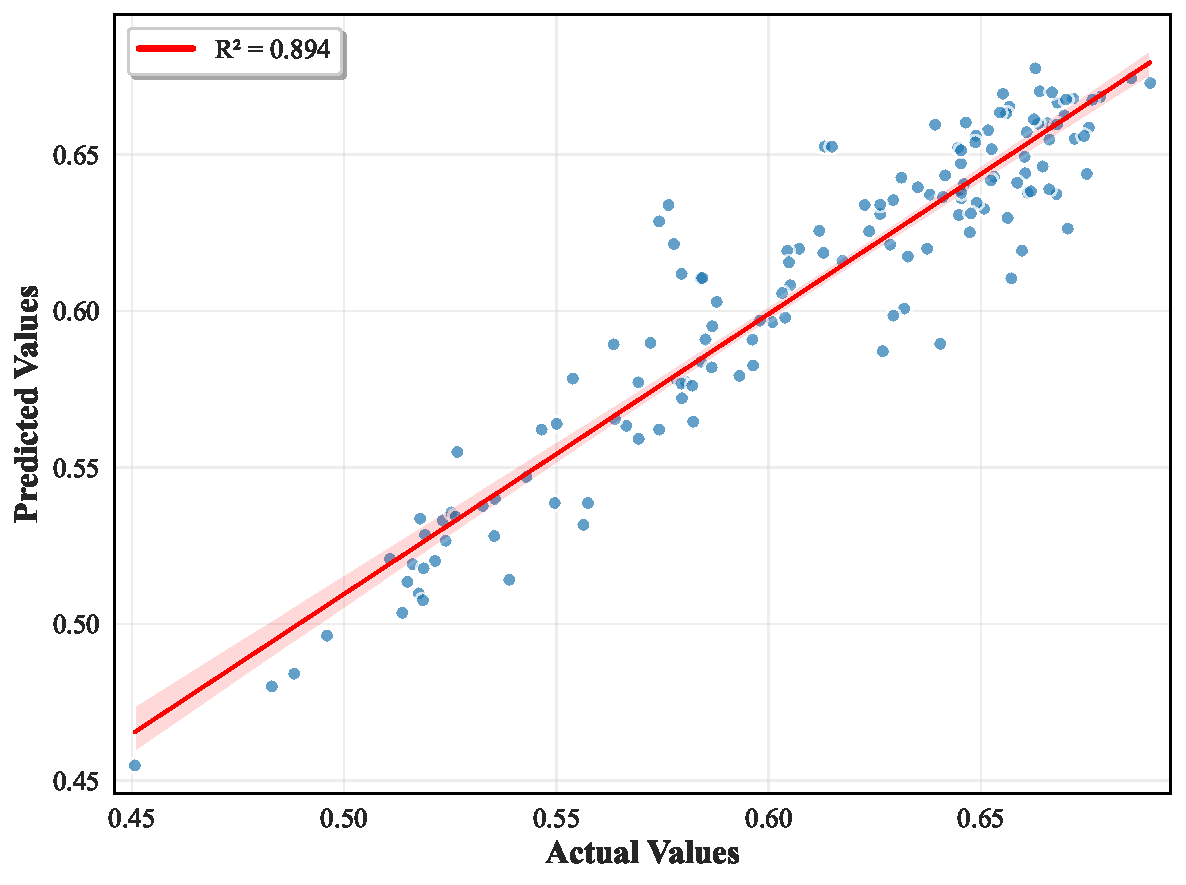
\includegraphics[height=1.7in]{./figs/Figure_9_a.pdf} & 
        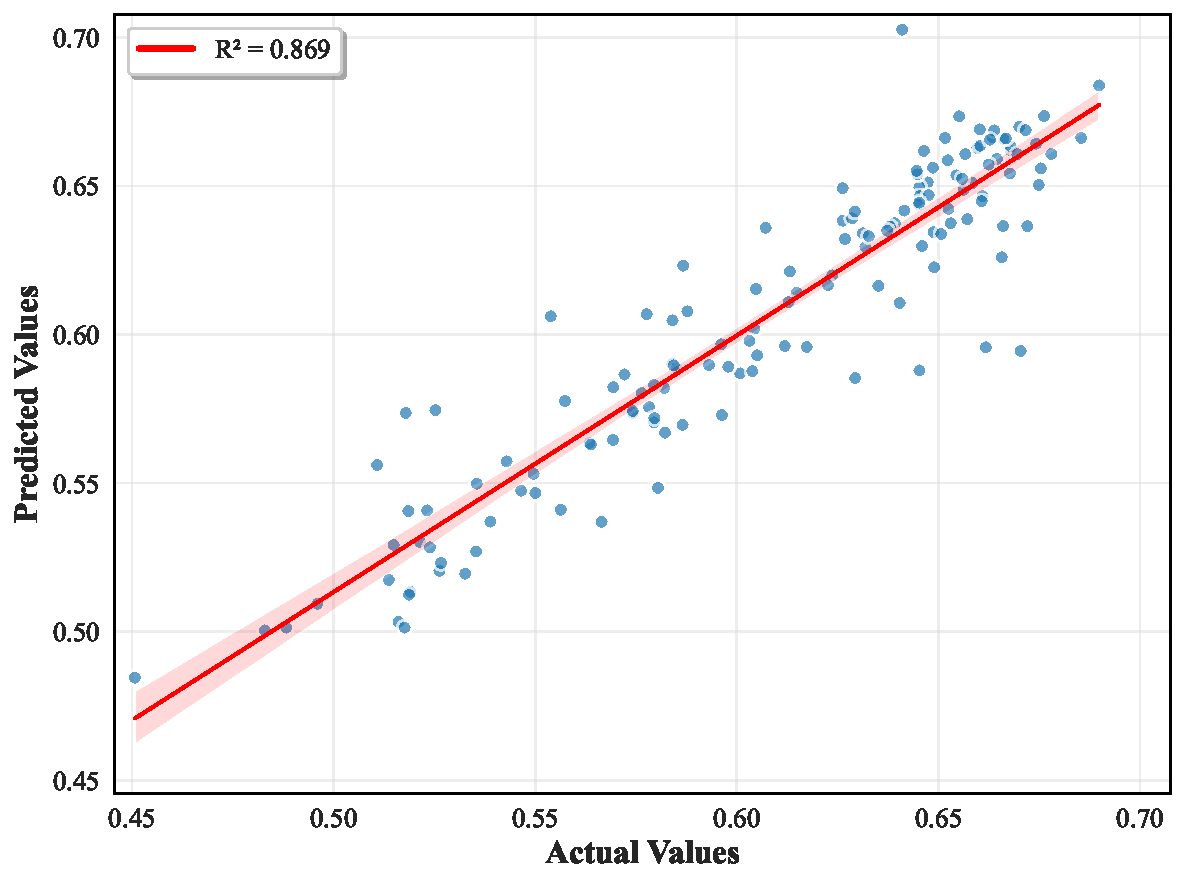
\includegraphics[height=1.7in]{./figs/Figure_9_b.pdf} \\ [-0.5pt]
        \scriptsize (a) $\nu$-SVR & 
        \scriptsize (b) Peephole \\ [4pt]
        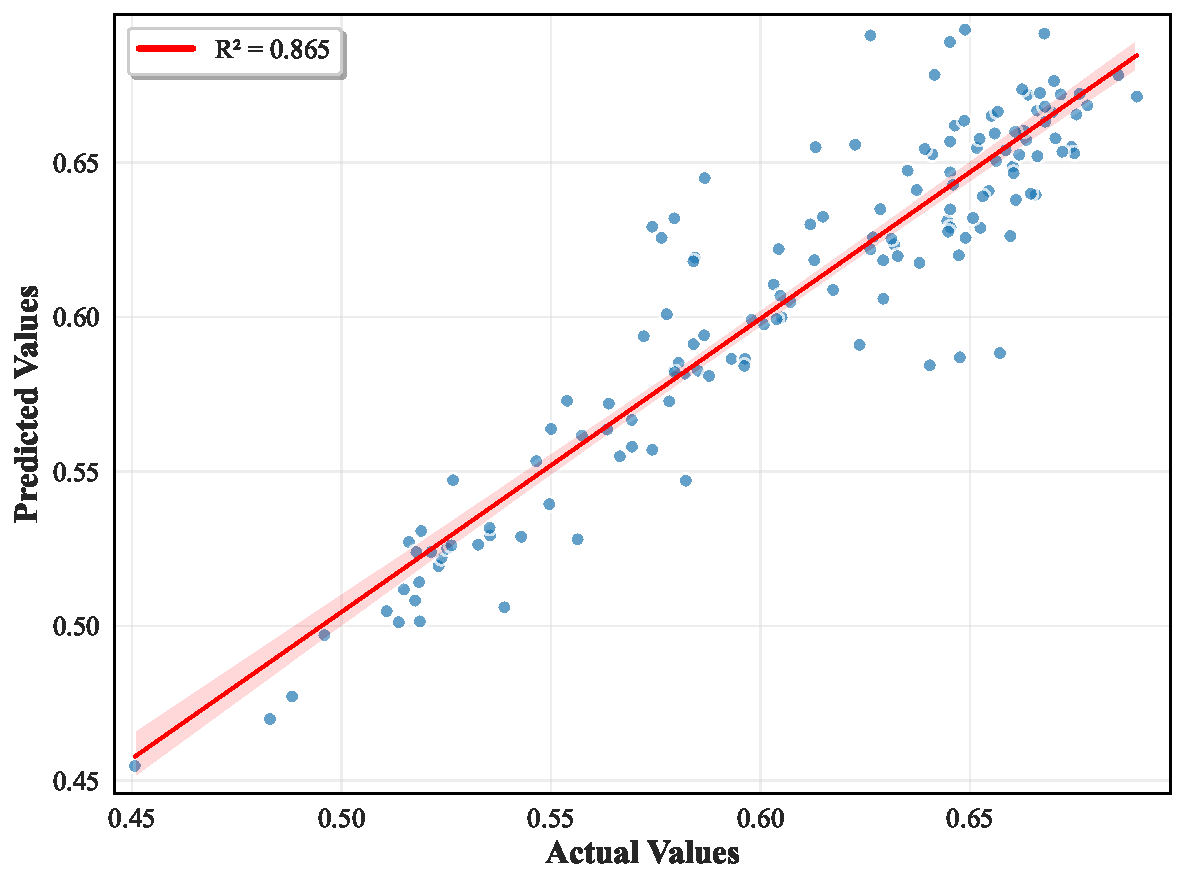
\includegraphics[height=1.7in]{./figs/Figure_9_c.pdf} & 
        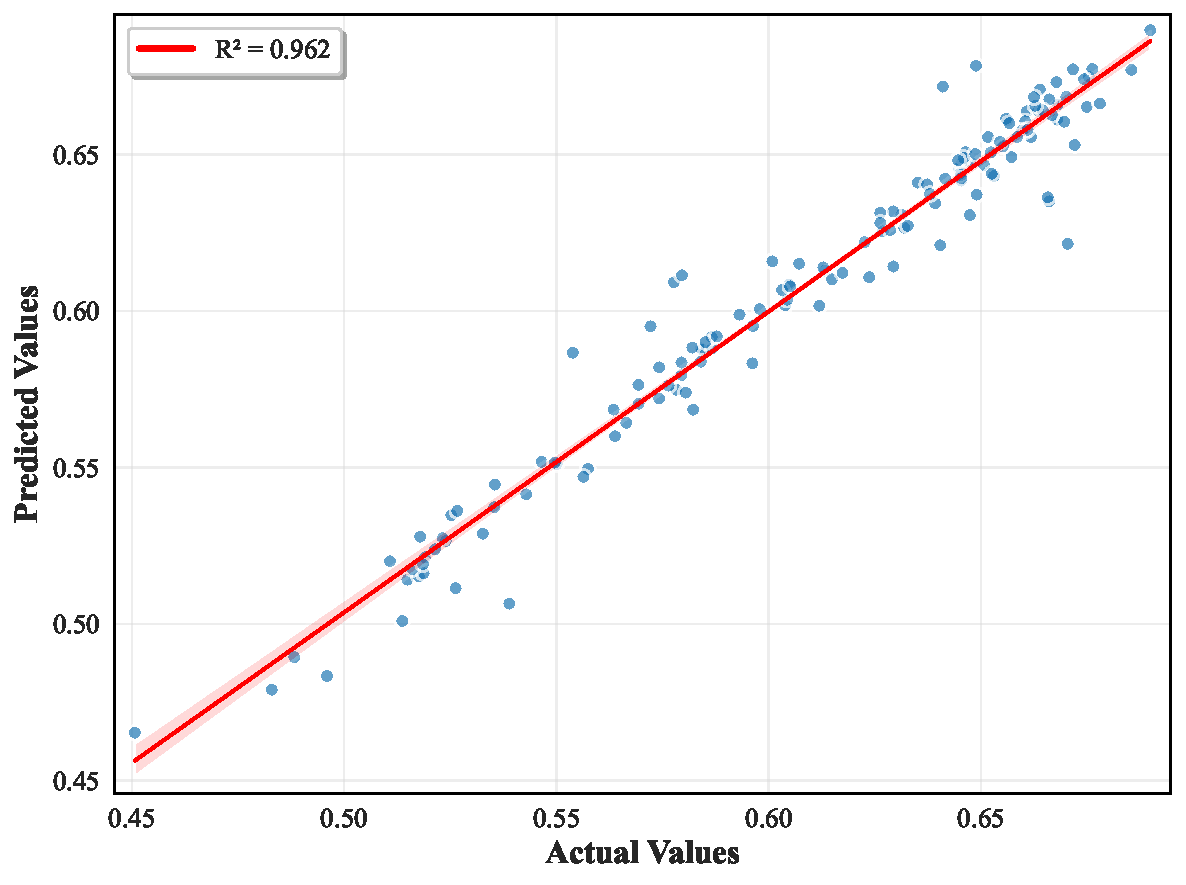
\includegraphics[height=1.7in]{./figs/Figure_9_d.pdf} \\
        \scriptsize (c) GCN & 
        \scriptsize (d) Ours
    \end{tabular}
    \caption{Accuracy prediction results, with fitted linear regressions shown in red and shaded 95\% confidence intervals.}\label{fig:9}
\end{figure}

Figure~\ref{fig:9} compares predicted accuracy with the measured short-training labels for CIF-Net and the baseline predictors. Points near the identity line $y=x$ indicate closer numerical agreement, while systematic departures indicate prediction bias across the accuracy range. CIF-Net's points clustered more closely around this line, whereas the baselines showed larger deviations, particularly in the middle of the accuracy range. This visual pattern is consistent with the lower MSE and higher rank correlation reported in the main manuscript. The fitted regression lines and confidence intervals summarize the prediction trends, complementing the quantitative comparison with a view of how errors are distributed across architectures.


\section{Comparison of Pareto frontiers}
\begin{figure}[H]
    \centering
    \begin{tabular}{cc}
        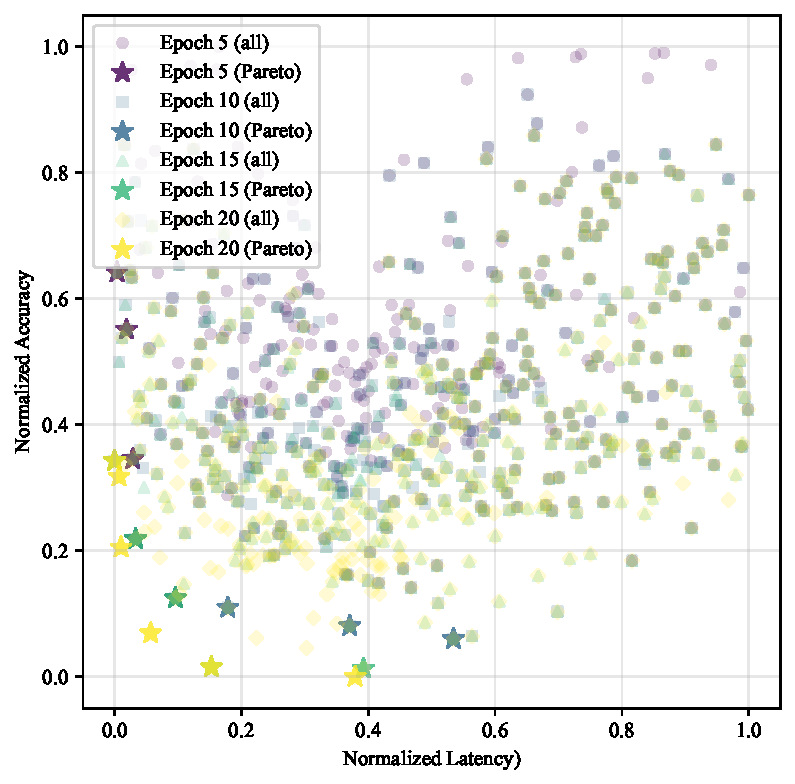
\includegraphics[height=2.2in]{./figs/Figure_10_a.pdf} & 
        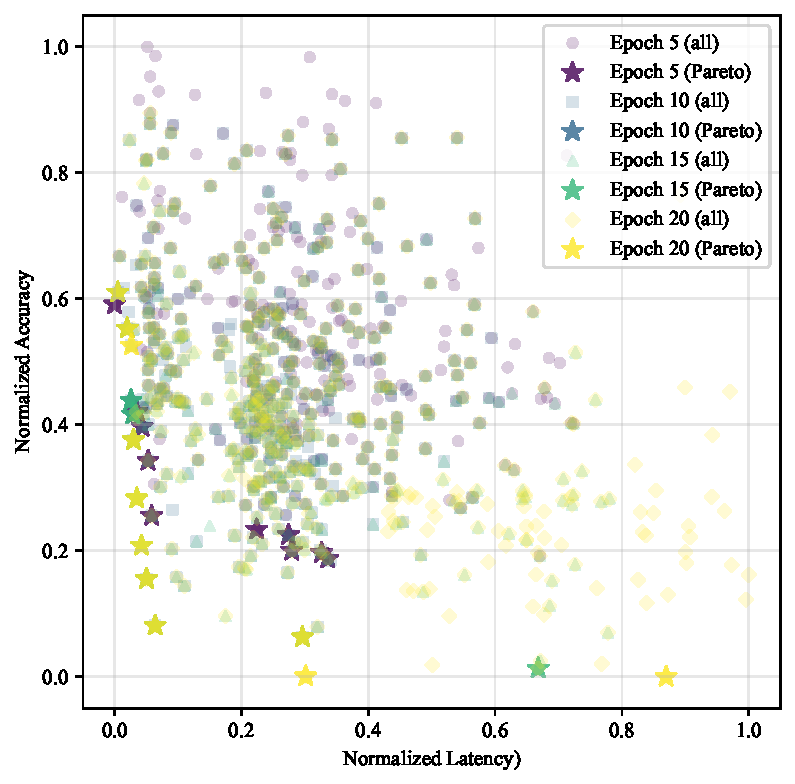
\includegraphics[height=2.2in]{./figs/Figure_10_b.pdf} \\ [-0.5pt]
        \scriptsize (a) One-stage  & 
        \scriptsize (b) Two-stage
    \end{tabular}
    \caption{One-stage and two-stage search trajectories, with latency measured at each evolutionary iteration for visualization. Two-stage exploration remains guided by accuracy--OPs, with platform-specific selection performed afterward.}\label{fig:10}
\end{figure}
Figure~\ref{fig:10} compares how the two search strategies explore accuracy--latency trade-offs. The one-stage baseline uses latency directly during evolution and explores a wider region, including many medium- and high-latency candidates. Two-stage search first screens architectures using accuracy and OPs, producing a candidate distribution concentrated nearer the low-latency boundary in this comparison. Its denser frontier shows how the initial screening narrows the region requiring platform-specific evaluation. The subsequent latency-aware choice is made after exploration, as specified in Algorithm~\ref{alg:flashnas}. Thus, the figure supports the role of OPs as a coarse exploration criterion under the evaluated setting, while the final deployment choice still depends on the target platform's latency.

\FloatBarrier
\section{\textcolor{red}{Architecture selection settings and accuracy--latency weight sensitivity}}
\label{sec:supp_selection_settings}
\subsection{\textcolor{red}{Stage-II accuracy--latency weight sensitivity}}
\label{sec:supp_weight_sensitivity}

\textcolor{red}{We examined the effect of the Stage-II weight on ImageNet-100 with the Cortex-X4 CPU by holding the Stage-I candidate set fixed and varying $w_{\mathrm{Lat}}\in\{0,0.25,0.5,0.75,1\}$. In Algorithm~\ref{alg:flashnas}, this coefficient weights normalized accuracy loss and $1-w_{\mathrm{Lat}}$ weights normalized latency. The endpoints therefore select for accuracy alone or latency alone within the same pool, while intermediate settings trade off the two objectives. Table~\ref{tab:8} reports the selected architectures' full-training accuracy and measured CPU latency, allowing the effect of final selection to be examined without rerunning Stage-I exploration.}

\begin{table}[!htbp]
\centering
\caption{\textcolor{red}{Stage-II weight sensitivity on ImageNet-100 for Cortex-X4 deployment, reporting full-training accuracy and measured latency per image. CPU latency is reported as mean $\pm$ SD over 50 timed iterations.}}
\small
\begin{tabular}{lcc}
\toprule[1.5pt]
$w_{\mathrm{Lat}}$ & Full-training Top-1 (\%) & Measured CPU latency (\textcolor{red}{ms/image}) \\
\midrule
0 &  80.33 &  $139.97\pm1.15$  \\
0.25 & 81.40 &  $164.57\pm1.37$  \\
0.5 & 81.40 & $164.57\pm1.37$ \\
0.75 & 81.81 &  $255.35\pm2.12$  \\
1 & 82.07 & $412.91\pm3.80$ \\
\bottomrule[1.5pt]

\end{tabular}
\label{tab:8}
\end{table}
% Record check: identify whether this particular sweep selected candidates
% using CLE predictions or direct measurements; reported measured latency
% alone does not establish which signal guided selection.

\textcolor{red}{Placing more weight on latency reduced inference time at a cost in accuracy. The accuracy-only endpoint reached 82.07\% Top-1 with 412.91\,ms/image latency, whereas $w_{\mathrm{Lat}}=0.5$ yielded 81.40\% at 164.57\,ms/image, matching FlashNAS-BNN-G. This corresponds to a 60.1\% latency reduction with Top-1 accuracy lower by 0.67 percentage points. Weights 0.25 and 0.5 produced the same reported performance point, consistent with a plateau when a continuous weight is applied to a discrete candidate pool; equal values alone do not identify the selected architecture. The accuracy-only endpoint also matched F's reported accuracy and CPU latency. F nevertheless has its own OPs-based selection setting in Table~\ref{tab:model_selection_config}, so this performance agreement does not establish that it underwent Stage-II selection.}

\FloatBarrier
\subsection{\textcolor{red}{Model-selection configurations}}
\label{sec:supp_model_selection}

\textcolor{red}{Table~\ref{tab:model_selection_config} distinguishes changes in the selection objective from changes in the target platform. A--F provide platform-independent reference variants selected using the accuracy--OPs objective, with $w_{\mathrm{OP}}$ weighting accuracy; F is the accuracy-oriented endpoint under its OP constraint. G/H/I apply the Stage-II accuracy--latency objective to CPU, GPU, and FPGA, respectively, with $w_{\mathrm{Lat}}$ weighting accuracy. Their common accuracy weight does not imply identical scoring, because each platform supplies a different latency input and its latency range is normalized separately. Accuracy normalization uses the corresponding candidate pool. Candidate reuse is therefore defined for a fixed dataset, search space, and search run, while platform-specific latency evaluation determines the final hardware-aware architecture.}

\begin{table}[H]
\centering
\linespread{1.0}\selectfont
\caption{\textcolor{red}{Selection objectives, trade-off weights, and target platforms for FlashNAS-BNN architecture variants. Model suffixes match the main manuscript; asterisks denote models searched from ReActNet-BiR18. N/A indicates that the corresponding selection objective was not used.}}
\label{tab:model_selection_config}
\small
\setlength{\tabcolsep}{3pt}
{\color{red}
\begin{tabularx}{\textwidth}{>{\raggedright\arraybackslash}p{0.10\textwidth} >{\raggedright\arraybackslash}p{0.19\textwidth} >{\raggedright\arraybackslash}X >{\raggedright\arraybackslash}p{0.13\textwidth} >{\raggedright\arraybackslash}p{0.18\textwidth}}
\toprule
\makecell[l]{Model\\suffix} & Dataset & Selection criterion & \makecell[l]{OPs\\selection\\$w_{\mathrm{OP}}$} & \makecell[l]{Stage II\\$w_{\mathrm{Lat}}$ / target} \\
\midrule
A$^*$ & CIFAR-10/100 & Accuracy--OPs selection & 0.25 & N/A \\
B$^*$ & CIFAR-10/100 & Accuracy--OPs selection & 0.50 & N/A \\
C$^*$ & CIFAR-10/100 & Accuracy--OPs selection & 0.75 & N/A \\
D & ImageNet-1000 & Accuracy--OPs selection & 0.50 & N/A \\
E & ImageNet-1000 & Accuracy--OPs selection & 0.75 & N/A \\
F & ImageNet-100 & Accuracy-only under OP constraint & 1.00 & N/A \\
G & ImageNet-100 & Stage-II accuracy--latency & N/A & 0.5 / CPU \\
H & ImageNet-100 & Stage-II accuracy--latency & N/A & 0.5 / GPU \\
I & ImageNet-100 & Stage-II accuracy--latency & N/A & 0.5 / FPGA \\
\bottomrule
\end{tabularx}}
\end{table}
% Record check: preserve run-specific candidate IDs, feasibility budgets, and
% normalization records. Equal rounded OPs for D/E do not establish a shared
% pool or dominance under the predictor used at selection time.

\FloatBarrier
\section{\textcolor{red}{Additional evaluation of CLE}}
\label{sec:supp_cle_evaluation}

\subsection{\textcolor{red}{Threshold selection for Stage-II latency evaluation}}

The threshold in Algorithm~\ref{alg:flashnas} balances the cost of directly measuring a candidate pool against the cost of fitting CLE and predicting its latencies. For small pools, direct evaluation avoids predictor-training overhead; as the pool grows, that overhead can be amortized over more candidates. Figure~\ref{fig:11} places the measured crossover near 250 candidates, motivating $N_{\mathrm{thr}}=250$ for the evaluated setup. The cost at this point is $\sum_i^{N_{init}}T_{inference}+T_{predict}^{train}-T_{stageI}=0.961+0.049-0.53=0.48$ GPU-hours. Direct measurement was less costly below the crossover, whereas CLE prediction was less costly above it, providing the operational basis for switching between the two latency-evaluation procedures.

\begin{figure}[H]
    \centering
    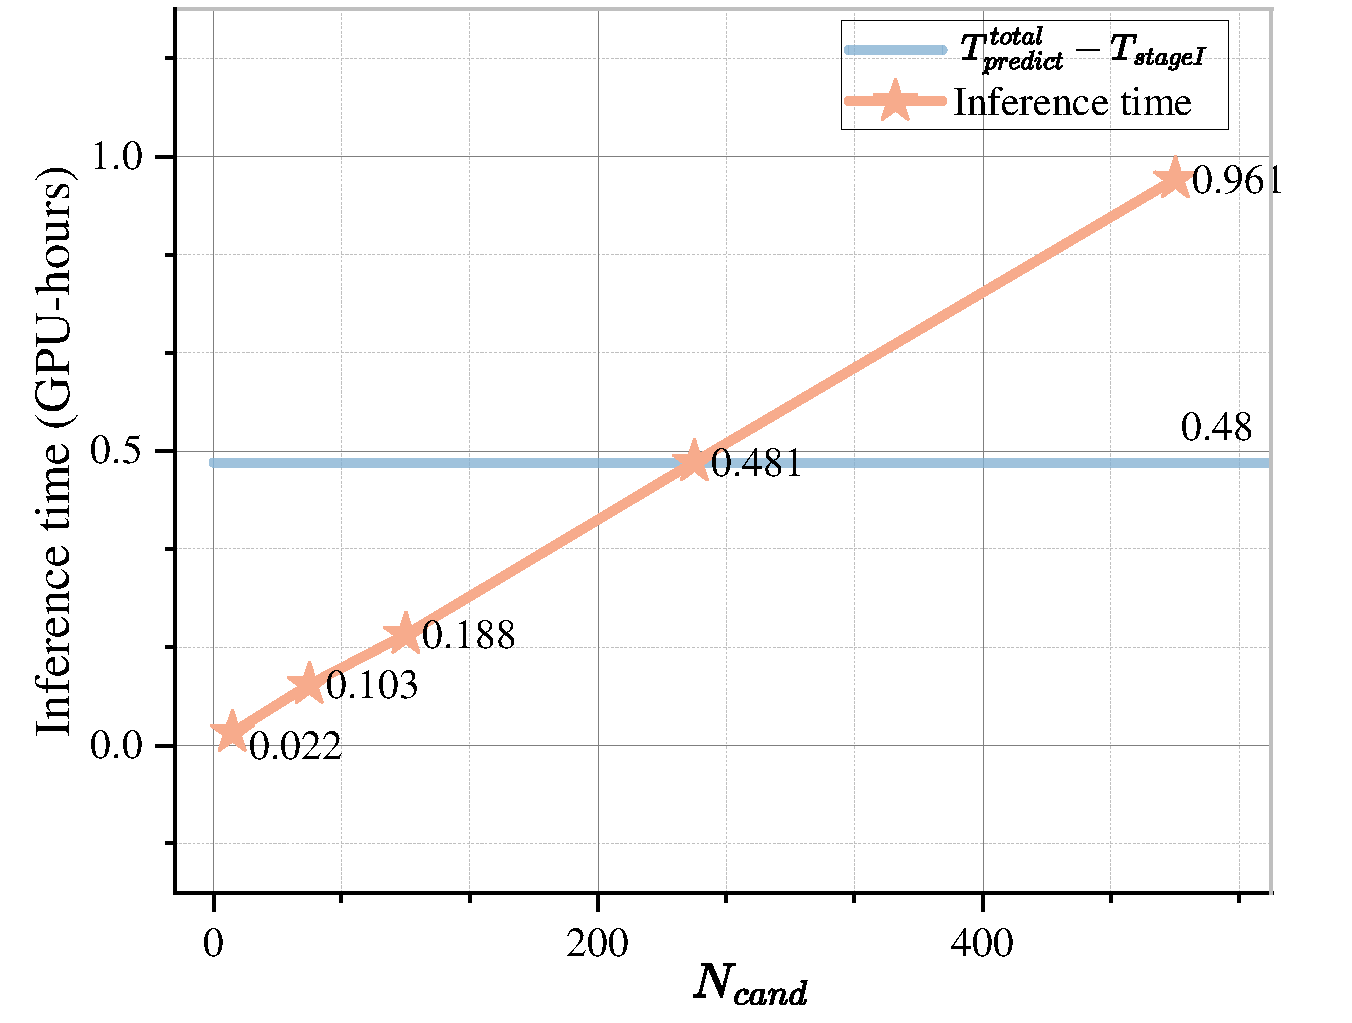
\includegraphics[width=0.6\columnwidth]{./figs/Figure_11.pdf}
    \caption{Inference time for different numbers of candidate architectures with and without CLE.}\label{fig:11}
\end{figure}

\subsection{\textcolor{red}{CLE performance over repeated searches}}
\label{sec:architecture_selection_repeatability}

\textcolor{red}{To assess whether latency estimation supports repeatable architecture selection, we compared CLE with OPs Proxy, $\nu$-SVR, BRP-NAS, CLCDLP, nn-Meter, and Actually measured on CPU, GPU, and FPGA. All methods used matched OP constraints and the latency-only Stage-II setting $w_{\mathrm{Lat}}=0$, separating this estimator comparison from the accuracy--latency settings used for G/H/I. Searches 1--3 used seeds 2024, 1234, and 42, respectively, with each seed fixed within its search. For each seed, OPs Proxy and CLE reused exactly the same candidate architectures. OPs Proxy ranked this shared pool by operation count, while CLE used estimated latency. Actually measured guided selection using hardware latency directly; the other methods used their respective estimates. We then measured the selected architectures using the protocol in Section~\ref{sec:detailed_latency_benchmark}. Table~\ref{tab:architecture_selection_repeatability} separates timing variation within each search from variation among the three search-specific mean latencies, and the main manuscript's error-bound percentages summarize the same searches.}

\begin{table}[H]
    \centering
    \linespread{1.0}\selectfont
    \caption{\textcolor{red}{Measured latencies of selected architectures in ms/image, reported as mean $\pm$ SD over 50 timed iterations per search. Overall reports the mean $\pm$ sample SD of the three search-specific mean latencies.}}
    \label{tab:architecture_selection_repeatability}
    \small
    \setlength{\tabcolsep}{2.5pt}
    {\color{red}
    \begin{tabular}{llcccc}
    \toprule
    Platform & Method & \makecell{Search 1\\(ms/image)} & \makecell{Search 2\\(ms/image)} & \makecell{Search 3\\(ms/image)} & \makecell{Overall\\(ms/image)} \\
    \midrule
    \multirow{7}{*}{CPU} & Actually measured & $139.88\pm1.07$ & $139.60\pm1.09$ & $140.43\pm1.08$ & $139.97\pm0.42$ \\
     & OPs Proxy & $150.11\pm1.29$ & $158.16\pm1.83$ & $147.07\pm1.32$ & $151.78\pm5.73$ \\
     & $\nu$-SVR & $147.85\pm1.56$ & $148.00\pm1.41$ & $142.90\pm1.22$ & $146.25\pm2.90$ \\
     & BRP-NAS & $146.12\pm1.47$ & $146.11\pm1.14$ & $144.30\pm1.31$ & $145.51\pm1.05$ \\
     & CLCDLP & $142.88\pm1.10$ & $144.18\pm1.21$ & $143.80\pm1.32$ & $143.62\pm0.67$ \\
     & nn-Meter & $142.57\pm1.14$ & $143.77\pm1.25$ & $142.24\pm1.09$ & $142.86\pm0.81$ \\
     & CLE & $141.39\pm1.38$ & $141.81\pm1.15$ & $140.76\pm1.25$ & $141.32\pm0.53$ \\
    \midrule
    \multirow{7}{*}{GPU} & Actually measured & $43.76\pm0.16$ & $43.83\pm0.16$ & $43.75\pm0.17$ & $43.78\pm0.04$ \\
     & OPs Proxy & $48.45\pm0.31$ & $44.14\pm0.24$ & $45.62\pm0.28$ & $46.07\pm2.19$ \\
     & $\nu$-SVR & $44.58\pm0.26$ & $44.96\pm0.23$ & $44.38\pm0.21$ & $44.64\pm0.29$ \\
     & BRP-NAS & $44.27\pm0.24$ & $43.88\pm0.17$ & $43.85\pm0.20$ & $44.00\pm0.23$ \\
     & CLCDLP & $44.40\pm0.25$ & $44.22\pm0.22$ & $44.13\pm0.18$ & $44.25\pm0.14$ \\
     & nn-Meter & $44.12\pm0.20$ & $44.38\pm0.22$ & $44.01\pm0.21$ & $44.17\pm0.19$ \\
     & CLE & $43.80\pm0.22$ & $44.03\pm0.25$ & $43.90\pm0.19$ & $43.91\pm0.12$ \\
    \midrule
    \multirow{7}{*}{FPGA} & Actually measured & $2.294\pm0.005$ & $2.301\pm0.006$ & $2.296\pm0.005$ & $2.297\pm0.004$ \\
     & OPs Proxy & $2.380\pm0.010$ & $2.475\pm0.012$ & $2.327\pm0.009$ & $2.394\pm0.075$ \\
     & $\nu$-SVR & $2.309\pm0.008$ & $2.318\pm0.009$ & $2.303\pm0.007$ & $2.310\pm0.008$ \\
     & BRP-NAS & $2.320\pm0.010$ & $2.304\pm0.008$ & $2.306\pm0.009$ & $2.310\pm0.009$ \\
     & CLCDLP & $2.327\pm0.009$ & $2.313\pm0.011$ & $2.320\pm0.008$ & $2.320\pm0.007$ \\
     & nn-Meter & $2.317\pm0.008$ & $2.304\pm0.007$ & $2.306\pm0.009$ & $2.309\pm0.007$ \\
     & CLE & $2.296\pm0.007$ & $2.306\pm0.008$ & $2.298\pm0.007$ & $2.300\pm0.005$ \\
    \bottomrule
    \end{tabular}}
\end{table}

\textcolor{red}{CLE yielded the lowest Overall mean latency and between-search SD among the six latency estimators on each platform (Table~\ref{tab:architecture_selection_repeatability}). Relative to Actually measured, its mean latency gaps were 1.35\,ms/image on CPU, 0.13\,ms/image on GPU, and 0.003\,ms/image on FPGA. These results connect latency prediction to the measured performance of the architectures ultimately selected, rather than evaluating prediction error alone. Across the three searches, CLE remained close to hardware-guided selection while showing less between-search variation than the other estimators. The small FPGA differences should be read alongside the timing and search variability in the table; these measurements do not establish statistical significance for such small gaps.}


\section{Structural intensity assumptions}
\label{sec:structural_intensity}
This section states analytical assumptions; it does not report additional hardware measurements. For a standard dense convolution with input dimensions $H_i\times W_i\times C_{\mathrm{in}}$, output dimensions $H_o\times W_o\times C_{\mathrm{out}}$, and kernel size $K$, count one multiply--accumulate as one structural operation:
\begin{align}
O &\approx H_oW_oC_{\mathrm{in}}C_{\mathrm{out}}K^2,\\
Q_{\mathrm{ideal}} &\approx b_{\mathrm{in}}H_iW_iC_{\mathrm{in}}
 + b_{\mathrm{out}}H_oW_oC_{\mathrm{out}}
 + b_w C_{\mathrm{in}}C_{\mathrm{out}}K^2,\\
I_{\mathrm{ideal}} &= O/Q_{\mathrm{ideal}}.
\end{align}
Here $b_{\mathrm{in}}$, $b_{\mathrm{out}}$, and $b_w$ denote effective storage bytes per element. The estimate assumes ideal reuse, counting each input, output, and weight element once; it omits additional traffic from padding materialization, intermediate buffers, and other implementation details. Unequal input and output spatial dimensions, including downsampling, must retain their respective dimensions in $Q_{\mathrm{ideal}}$.

With equal spatial dimensions and equal storage cost, removing the common per-element byte factor gives the structural proxy in the main manuscript. Only under activation dominance, $HW(C_{\mathrm{in}}+C_{\mathrm{out}})\gg C_{\mathrm{in}}C_{\mathrm{out}}K^2$, does it simplify to $C_{\mathrm{in}}C_{\mathrm{out}}K^2/(C_{\mathrm{in}}+C_{\mathrm{out}})$, and only with equal channels does this become $C_iK^2/2$.

Neither $Q_{\mathrm{ideal}}$ nor the structural proxy measures device traffic. BNN packing, buffering, accumulation, and operator fusion can change actual data movement. A device Roofline requires operation counts and transferred bytes at a specified memory interface, consistent with its throughput and bandwidth bounds. Figure 4(a) in the main manuscript is FPGA-specific; no additional CPU/GPU Roofline validation is claimed here. These expressions motivate searching kernel size and width rather than replace CLE or measured latency.

\FloatBarrier
\bibliographystyle{elsarticle-num}
\bibliography{cas-refs}

\end{document}
